\section{Aufnahmen}

\begin{figure}
  \centering
  \label{fig:anfangssignal_ohne_rausch}
  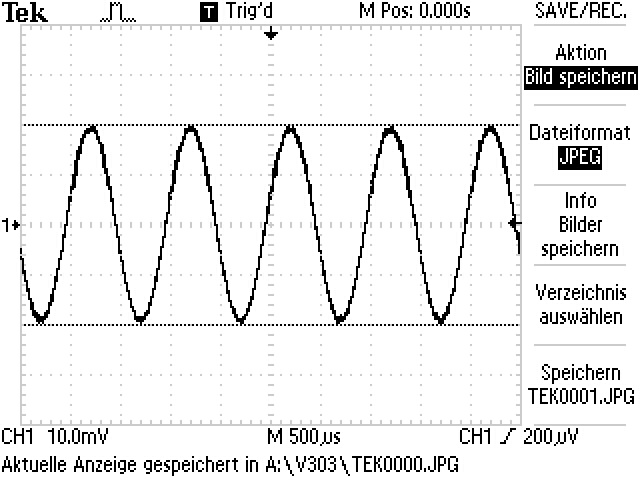
\includegraphics{aufnahmen/eingangssignal.pdf}
  \caption{Vom Funktionsgenerator erzeugte Sinusspannung}
\end{figure}

\begin{figure}
  \centering
  \label{fig:referenzsignal_ohne_rausch}
  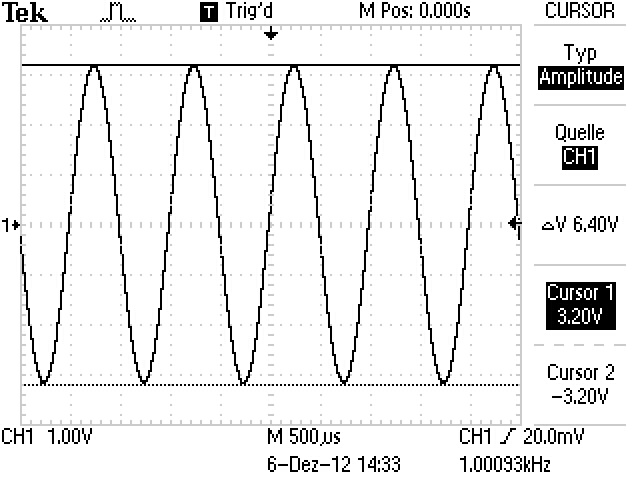
\includegraphics{aufnahmen/referenzsignal.pdf}
  \caption{Vom Funktionsgenerator erzeugtes Referenzsignal}
\end{figure}


\begin{figure}
  \centering
  \label{fig:phase_0_nicht_verrauscht}
  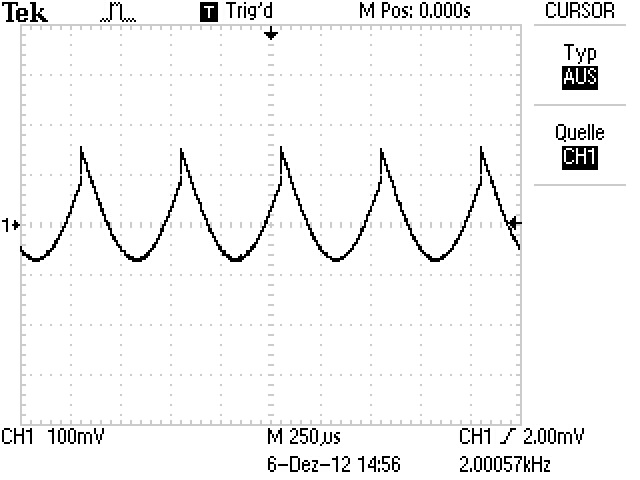
\includegraphics{aufnahmen/phase_0_ohne_rauschen.pdf}
  \caption{Nicht verrauschtes Mischsignal bei eingestellter
    Phasenverschiebung von \SI{0}{\degree}}
\end{figure}


\begin{figure}
  \centering
  \label{fig:phase_45_nicht_verrauscht}
  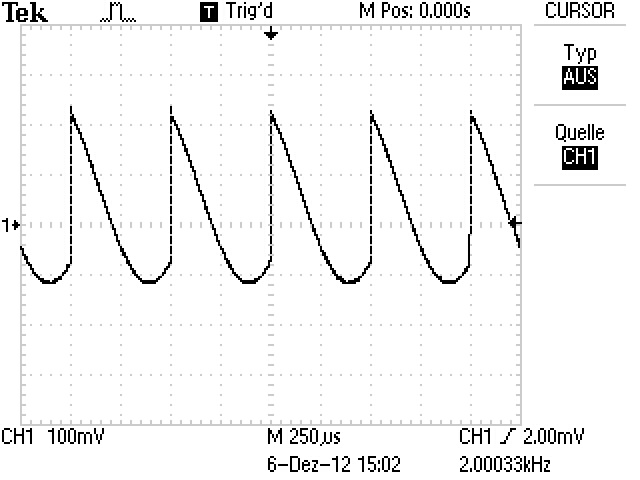
\includegraphics{aufnahmen/phase_45_ohne_rauschen.pdf}
  \caption{Nicht verrauschtes Mischsignal bei eingestellter
    Phasenverschiebung von \SI{45}{\degree}}
\end{figure}


\begin{figure}
  \centering
  \label{fig:phase_90_nicht_verrauscht}
  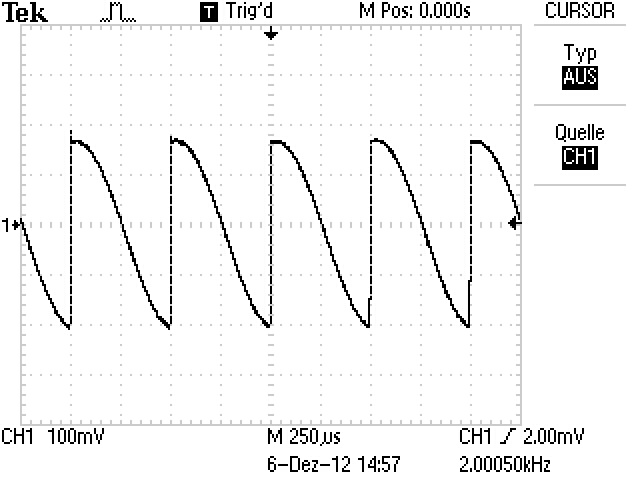
\includegraphics{aufnahmen/phase_90_ohne_rauschen.pdf}
  \caption{Nicht verrauschtes Mischsignal bei eingestellter
    Phasenverschiebung von \SI{90}{\degree}}
\end{figure}


\begin{figure}
  \centering
  \label{fig:phase_180_nicht_verrauscht}
  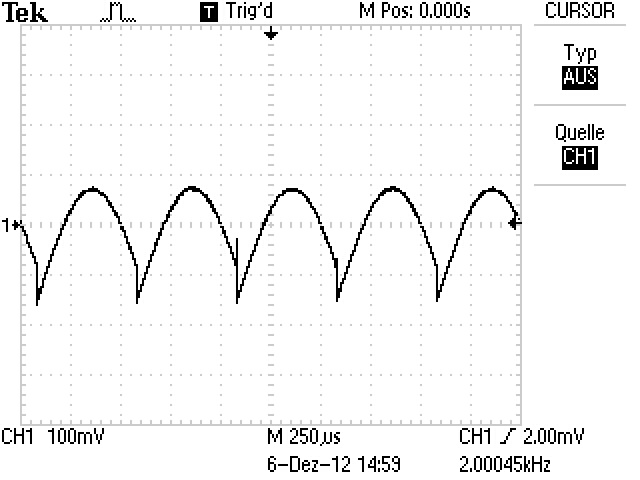
\includegraphics{aufnahmen/phase_180_ohne_rauschen.pdf}
  \caption{Nicht verrauschtes Mischsignal bei eingestellter
    Phasenverschiebung von \SI{180}{\degree}}
\end{figure}


\begin{figure}
  \centering
  \label{fig:phase_270_nicht_verrauscht}
  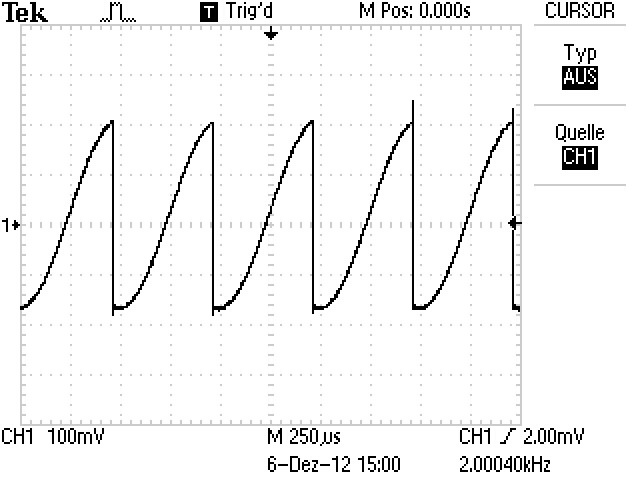
\includegraphics{aufnahmen/phase_270_ohne_rauschen.pdf}
  \caption{Nicht verrauschtes Mischsignal bei eingestellter
    Phasenverschiebung von \SI{270}{\degree}}
\end{figure}


\begin{figure}
  \centering
  \label{fig:gleichspannung_ohne_rausch}
  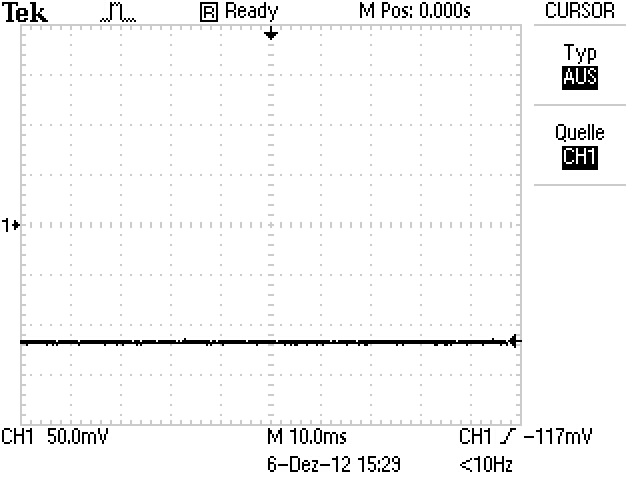
\includegraphics{aufnahmen/gleichspannung_ohne_rauschen.pdf}
  \caption{Ausgangssignal des Lock-In-Verstärkers bei nicht verrauschtem
    Eingangssignal}
\end{figure}


\begin{figure}
  \centering
  \label{fig:vollrausch}
  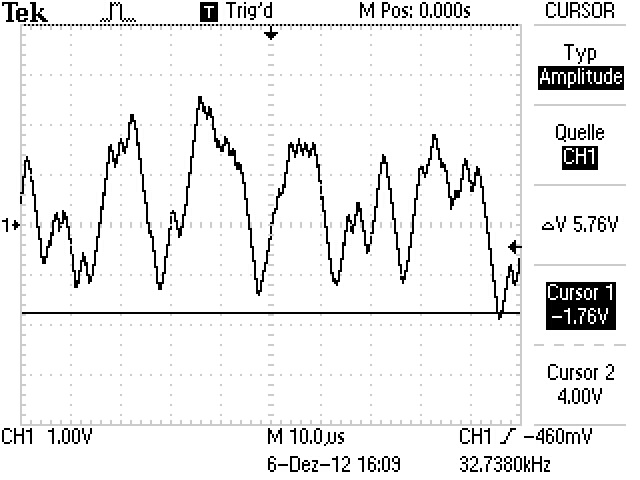
\includegraphics{aufnahmen/vollrausch.pdf}
  \caption{Verrauschtes Eingangssignal}
\end{figure}

\begin{figure}
  \centering
  \label{fig:bandrausch}
  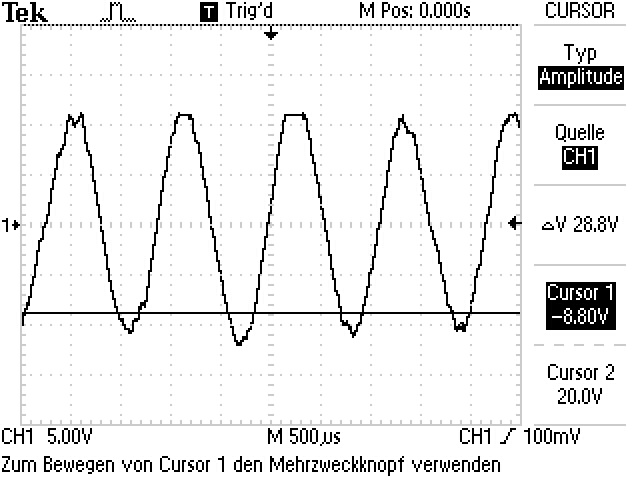
\includegraphics{aufnahmen/bandrausch.pdf}
  \caption{Form des verrauschten Signales nach Bandpassfilter}
\end{figure}

\begin{figure}
  \centering
  \label{fig:phase_0_verrauscht}
  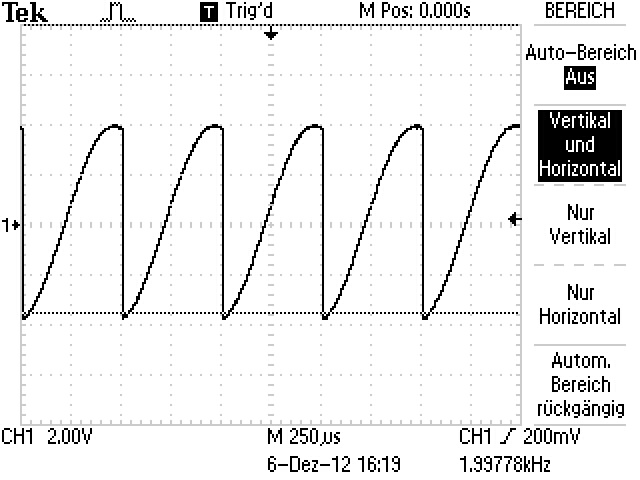
\includegraphics{aufnahmen/phase_0_verrauscht.pdf}
  \caption{Verrauschtes Mischsignal bei eingestellter Phasenverschiebung
    von \SI{0}{\degree}}
\end{figure}

\begin{figure}
  \centering
  \label{fig:phase_45_verrauscht}
  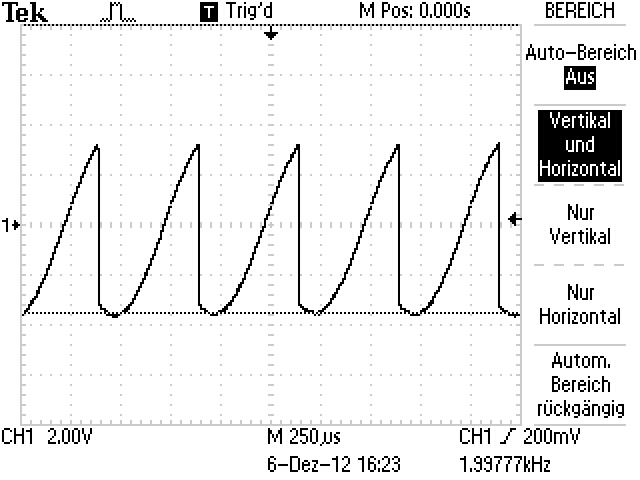
\includegraphics{aufnahmen/phase_45_verrauscht.pdf}
  \caption{Verrauschtes Mischsignal bei eingestellter Phasenverschiebung
    von \SI{45}{\degree}}
\end{figure}

\begin{figure}
  \centering
  \label{fig:phase_90_verrauscht}
  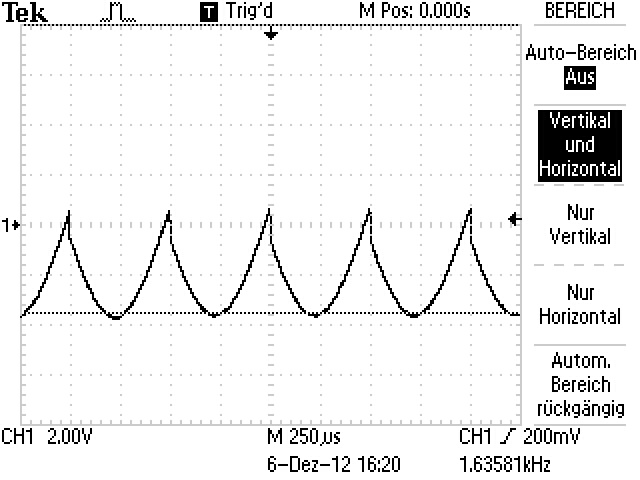
\includegraphics{aufnahmen/phase_90_verrauscht.pdf}
  \caption{Verrauschtes Mischsignal bei eingestellter Phasenverschiebung
    von \SI{90}{\degree}}
\end{figure}

\begin{figure}
  \centering
  \label{fig:phase_180_verrauscht}
  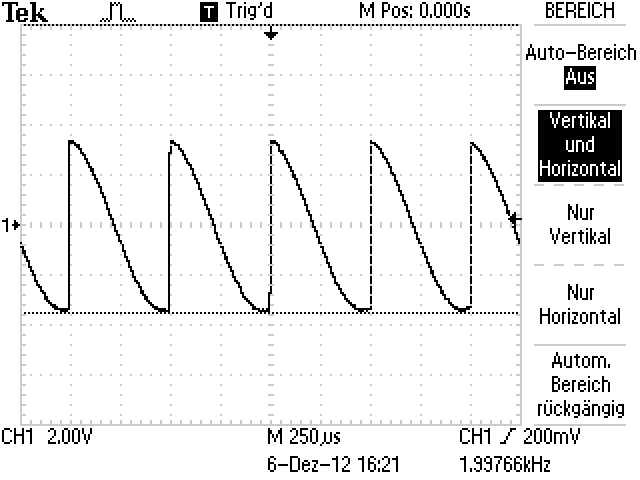
\includegraphics{aufnahmen/phase_180_verrauscht.pdf}
  \caption{Verrauschtes Mischsignal bei eingestellter Phasenverschiebung
    von \SI{180}{\degree}}
\end{figure}

\begin{figure}
  \centering
  \label{fig:phase_270_verrauscht}
  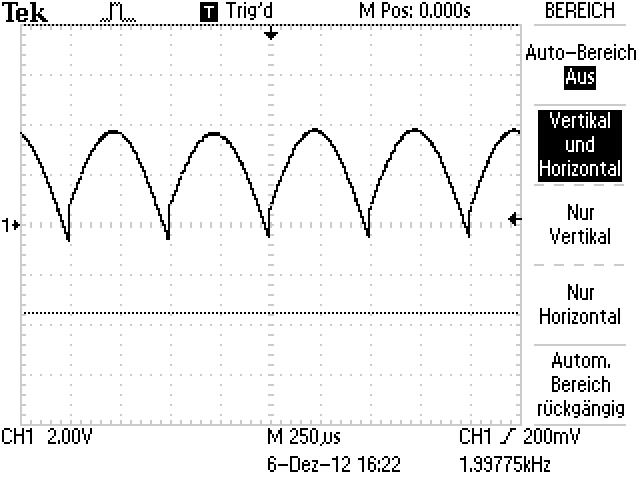
\includegraphics{aufnahmen/phase_270_verrauscht.pdf}
  \caption{Verrauschtes Mischsignal bei eingestellter Phasenverschiebung
    von \SI{270}{\degree}}
\end{figure}
